\documentclass{ximera}

\newcommand{\RR}{\mathbb R}
\renewcommand{\d}{\,d}
\newcommand{\dd}[2][]{\frac{d #1}{d #2}}
\renewcommand{\l}{\ell}
\newcommand{\ddx}{\frac{d}{dx}}
\newcommand{\dfn}{\textbf}
\newcommand{\eval}[1]{\bigg[ #1 \bigg]}


\author{Jim Fowler and Bart Snapp}
\title{A table of values}
\begin{document}

\begin{abstract}
Given a table of values, find approximations.
\end{abstract}

Let $F:\R^2\to\R$ be a differentiable function that is roughly
described by the following table of values.

\begin{center}
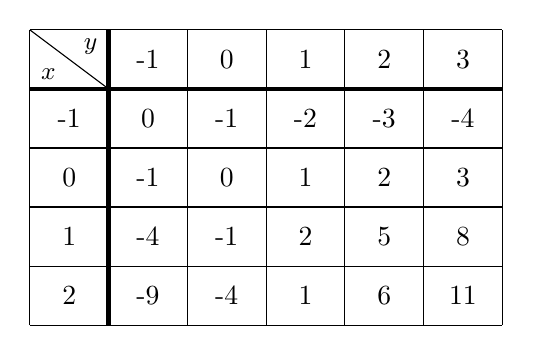
\begin{tikzpicture}[x=1cm,y=.75cm]
  \draw (0,0) grid [step=1] (6,5);
  
  \draw[ultra thick] (0,4)--(6,4);
  \draw[ultra thick] (1,0)--(1,5);
  
  \draw (0,5) -- (1,4);
  \node at (.9,4.9) [below left,inner sep=1pt] {\small$y$};
  \node at (0.1,4.1) [above right,inner sep=1pt] {\small$x$};
  
  %% x-values
  \node at (0.5,3.5) { -1 };
  \node at (0.5,2.5) { 0 };
  \node at (0.5,1.5) { 1 };
  \node at (0.5,0.5) { 2 };
  
  %% y-values
  \node at (1.5,4.5) { -1 };
  \node at (2.5,4.5) { 0 };
  \node at (3.5,4.5) { 1 };
  \node at (4.5,4.5) { 2 };
  \node at (5.5,4.5) { 3 };
  
  %% z-values
  %% top row
  \node at (1.5,3.5) {0};
  \node at (2.5,3.5) {-1};
  \node at (3.5,3.5) {-2};
  \node at (4.5,3.5) {-3};
  \node at (5.5,3.5) {-4};
  
  %% second row
  \node at (1.5,2.5) {-1};
  \node at (2.5,2.5) {0};
  \node at (3.5,2.5) {1};
  \node at (4.5,2.5) {2};
  \node at (5.5,2.5) {3};
  
  %% third row
  \node at (1.5,1.5) {-4};
  \node at (2.5,1.5) {-1};
  \node at (3.5,1.5) {2};
  \node at (4.5,1.5) {5};
  \node at (5.5,1.5) {8};
  
  %% bottom row
  \node at (1.5,.5) {-9};
  \node at (2.5,.5) {-4};
  \node at (3.5,.5) {1};
  \node at (4.5,.5) {6};
  \node at (5.5,.5) {11};
\end{tikzpicture}
\end{center}

\begin{exercise}
What is the value of $F(0,1)$?
\begin{prompt}
\[
  F(0,1) = \answer{-2}
\]
\end{prompt}
\end{exercise}

\begin{exercise}
Estimate $F^{(1,0)}(0,1)$ as we did in the textbook.
\begin{prompt}
\[
  F^{(1,0)}(0,1) = \answer{2}
\]
\end{prompt}
\end{exercise}

\begin{exercise}
Estimate $F^{(1,0)}(0,1)$ as we did in the textbook.
\begin{prompt}
\[
  F^{(1,0)}(x,y) = \answer{1}
\]
\end{prompt}
\end{exercise}

\begin{exercise}
Let $z = F(x,y)$ and compute $\d z$  at the point $(0,1)$ in terms of the estimated values of $\d x$ and  $\d y$.
\begin{prompt}
\[
  \d z = \answer{2 dx + 1 dy}
\]
\end{prompt}
\end{exercise}

\begin{exercise}
Use $\d z$ to estimate $F(0.5,1.5)$. 
\begin{prompt}
\[
  F(0.5,1.5) \approx \answer{5 + 0.5 \cdot 2 + 0.5 \cdot 1}.
\]
\end{prompt}
\end{exercise}

\begin{exercise}
Find an equation for a tangent plane for $F(x,y)$ at the point $(0,1)$.
\begin{prompt}
\[
z = \answer{(x - 0) \cdot 2 + (y - 1) \cdot 1}
\]
\end{prompt}
\end{exercise}

\begin{exercise}
Use your tangent plane to estimate $F(0.5,1.5)$. 
\begin{prompt}
\[
  F(0.5,1.5) \approx \answer{f + 0.5 \cdot 2 + 0.5 \cdot 1}.
\]
\end{prompt}
\end{exercise}

\begin{exercise}
Estimate the vector $\grad F(0,1)$.
\begin{prompt}
\[
  \grad F(0,1) \approx \vector{2,1}.
\]
\end{prompt}
\end{exercise}
% Emacs 25.2.1 (Org mode 8.2.10)
\end{document}